\title{Properties of Matrix Multiplication}
\subtitle{\SubTitleName}
\institute[]{\Course}
\author{\Instructor}
\maketitle


\tikzstyle{startstop} =[trapezium, trapezium left angle=70, trapezium right angle=110, minimum width=1cm, minimum height=1cm, text centered, fill=Teal!30]

\tikzstyle{io} = [trapezium, trapezium left angle=70, trapezium right angle=110, minimum width=1cm, minimum height=1cm, text centered, fill=DarkRed!30]

\tikzstyle{process} = [trapezium, trapezium left angle=70, trapezium right angle=110, minimum width=1cm, minimum height=1cm, text centered, fill=Gold!60]

\tikzstyle{arrow} = [thick,->,>=stealth]

\frame{\frametitle{Motivation}

    When $x$ and $y$ are real numbers, algebra can simplify equations that they involve. \pause For example: 
    \pause 
    \begin{itemize}
        \item If $xy=4y$ and $y\ne0$, then $x=4$. 
        \item For any real numbers $x$ and $y$, we can use $xy = yx$
    \end{itemize}
    \pause 
    Can we make similar statements with matrices? 
    \pause 

    \vspace{12pt}
    
    \Emph{Objectives}\\
        
    \begin{itemize}

        \item determine whether the multiplication of two matrices is defined

        \item apply algebraic properties of matrix multiplication to simplify and analyze matrix equations
        
    \end{itemize}


}

\frame{\frametitle{Matrix Dimensions and Matrix Multiplication}

    \pause The dimensions of $A$ and $B$ determine whether $AB$ is defined, \pause and what its dimensions will be.
    \pause 
    
    \begin{center}
        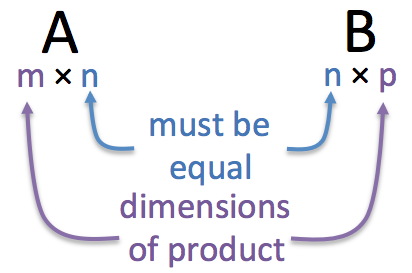
\includegraphics[width=0.3\textwidth]{Chapter2/images/matrix_multi2} 
    \end{center}

}


\frame{\frametitle{Example}

    Suppose $A$ is $3\times 5$ and $B$ is $5\times7$. Then:
    \begin{itemize}
        \item<2-> $AB$ is defined and the result is \onslide<3->{$3\times 7$}
        \item<4-> $BA$ is not defined \onslide<5->{because the number of columns of $B$ is not equal to the number of rows of $A$. }
    \end{itemize}

}


\frame{\frametitle{Properties of Matrix Multiplication} 

    \onslide<2->{$ A, B, C$ are matrices with sizes needed for matrix multiplication to be defined. }
    
    \begin{enumerate}
        \item<3-> (Associative)  $(AB)C= A (BC)$ 
        \item<4-> (Left Distributive)  $A (B+C) = AB + AC $ 
        \item<4-> (Right Distributive) $(A + B)C = AC + BC $ 
        \item<5-> (Identity)  $ I _{m} A = A I _{n}$, where $A$ is $m\times n$
    \end{enumerate}

    \onslide<6->{
    \Emph{\color{Teal}Warnings:}  
    }
    \begin{enumerate}
        \item<7->  (non-commutative) In general, $ AB \neq BA $. \pause  
        \item<8->  (non-cancellation) $ AB = A C $ does not mean $ B=C$. \pause 
        \item<9->  (Zero divisors) $ AB = 0$ does not mean that either $ A=0$ or $ B=0$.  
    \end{enumerate}
}

\frame{\frametitle{Example: Non-Commutative}
    Give an example of a matrix that does not commute with $A = \begin{pmatrix} 1&0\\0&0 \end{pmatrix}$.

    \vspace{12pt}
    \onslide<2->{\Emph{Solution} \\ We will create a $2\times 2$ matrix $B$, check whether $AB\ne BA$, } \onslide<3->{and if $AB\ne BA$, we have completed our task.}
    \begin{itemize}
        \item<4-> For simplicity, make most entries of $B$ equal to 0 or 1.
        \item \onslide<5->{ We can try: $B= \begin{pmatrix}0&0\\0&0\end{pmatrix}$.  But $AB=BA$ in this case. }
        \item \onslide<6->{ We can try: $B= \begin{pmatrix}1&0\\0&1\end{pmatrix}$.  But $AB=BA$ in this case. }
        \item<7-> What else can we try? 
    \end{itemize}
}



\frame{\frametitle{Example: Non-Commutative}
    Give an example of a matrix that does not commute with $A = \begin{pmatrix} 1&0\\0&0 \end{pmatrix}$.

    \vspace{12pt}
    \onslide<1->{\Emph{Solution}} \\ \onslide<2->{ Let's try: $B= \begin{pmatrix}
        0&1\\0&0
    \end{pmatrix}$. }
    \begin{align*}
        \onslide<3->{AB &= }\onslide<3->{\begin{pmatrix} 1&0\\0&0\end{pmatrix}\begin{pmatrix} 0&1\\0&0 \end{pmatrix} = \begin{pmatrix} 0&1\\0&0 \end{pmatrix}}\\
        \onslide<4->{BA &= }\onslide<5->{\begin{pmatrix} 0&1\\0&0 \end{pmatrix} \begin{pmatrix} 1&0\\0&0\end{pmatrix} = \begin{pmatrix} 0&0\\0&0 \end{pmatrix}}
    \end{align*}
    \onslide<6->{$AB\ne BA$, so $A$ and $B$ do not commute. }
}

\frame{\frametitle{Example: Non-Cancellation}
    Suppose $A = \begin{pmatrix} 1&0\\0&0 \end{pmatrix}$. Construct any non-zero matrices $B$ and $C$ so that $B\ne C$ but $AB=AC$.
    
    \vspace{4pt}
    \onslide<2->{\Emph{Solution} \\ We will create $2\times 2$ matrices $B$ and $C$,} \onslide<3->{with $B\ne C$, } \onslide<4->{and see if $AB = AC$.}\onslide<5->{ Let's try: $B= \begin{pmatrix}
        0&0\\1&0
    \end{pmatrix}$, and $C = \begin{pmatrix} 0&0\\0&1 \end{pmatrix}$. } 
    \begin{align*}
        \onslide<6->{AB &= }\onslide<6->{\begin{pmatrix} 1&0\\0&0\end{pmatrix}\begin{pmatrix} 0&0\\1&0 \end{pmatrix} = \begin{pmatrix} 0&0\\0&0 \end{pmatrix}}\\
        \onslide<7->{AC &= }\onslide<7->{\begin{pmatrix} 1&0\\0&0 \end{pmatrix} \begin{pmatrix} 0&0\\0&1\end{pmatrix} = \begin{pmatrix} 0&0\\0&0 \end{pmatrix}}
    \end{align*}
    \onslide<8->{$AB = AC$ and $B\ne C$ as needed. }    
}


\frame{\frametitle{The Associative Property} 

    If $C = \vec x$, then the associative property is: \onslide<2->{ $(AB)\vec x = A (B \vec x)$.}\onslide<3->{ Schematically: }
    
    \vspace{18pt}
    \onslide<4->{
    \begin{tikzpicture}[node distance=2cm]
        \onslide<4->{\node(x)  [startstop] {$\vec x$};}
        \onslide<5->{\node(abx)[process, right of=x,xshift=4cm]{$AB\vec x$};}
        \onslide<5->{\draw [arrow] (x) --node[anchor=south] {\small  \ \ \ multiply by $AB$} (abx);}   
        \onslide<6->{\node(bx) [io, below of=x] {$B\vec x$};}
        \onslide<6->{\draw [arrow] (x) -- node[anchor=east] {\small multiply by $B$} (bx);}
        \onslide<7->{\draw [arrow] (bx) -- node[anchor=north,xshift=1.2cm] {\small multiply by $A$} (abx);}
    \end{tikzpicture}
    }
    
    \vspace{4pt}
    
    \onslide<8->{The product $ AB\vec x$ can be obtained by either: multiplying by matrix $AB$, or by $B$ then by $A$. }
}




\begin{frame}
\frametitle{Associative Property Example}

    Suppose we want to rotate and scale a vector $\vec x$, \pause using transform $T(\vec x)$, where \pause

    \begin{align*}
        T(\vec x) &= A\vec x = A_rA_s \vec x\\
        A_r &= \begin{pmatrix} 0&-1\\1&0 \end{pmatrix} \\
        A_s &= \begin{pmatrix} 2&0\\0&2 \end{pmatrix}
    \end{align*}

\end{frame}

\begin{frame}
\frametitle{Associative Property Example Solution}

    By the associative property: 

    \begin{align*}
        T(\vec x) &= \left(A_rA_s\right) \vec x \onslide<2->{= \left(\begin{pmatrix} 0&-1\\1&0 \end{pmatrix} \begin{pmatrix} 2&0\\0&2 \end{pmatrix} \right) \begin{pmatrix} 1\\1 \end{pmatrix} = \begin{pmatrix} 0&-2\\2&0 \end{pmatrix}\begin{pmatrix} 1\\1 \end{pmatrix} = \begin{pmatrix} -2\\2 \end{pmatrix}} \\
        T(\vec x) &= A_r\left(A_s \vec x \right) \onslide<3->{= \begin{pmatrix} 0&-1\\1&0 \end{pmatrix} \left( \begin{pmatrix} 2&0\\0&2 \end{pmatrix}  \begin{pmatrix} 1\\1 \end{pmatrix} \right) = \begin{pmatrix} 0&-1\\1&0 \end{pmatrix}\begin{pmatrix} 2\\2 \end{pmatrix} = \begin{pmatrix} -2\\2 \end{pmatrix}}
    \end{align*}
    \onslide<4->{The end result is the same vector either way. }

\end{frame}

\frame{\frametitle{Summary}

    \begin{itemize}\setlength{\itemsep}{8pt}
        \item We used matrix dimensions to determine whether a matrix product is defined and what the dimensions of the product will be.\pause 
        \item We applied properties of matrix algebra to analyze matrix equations.
    \end{itemize}
    \vspace{4pt}
    
}

\frame{
}

\frame{
}
